%%%%%%%%%%%%%%%%%%%%%%%%%%%%%%%%%%%%%%%%%
% Masters/Doctoral Thesis 
% LaTeX Template
% Version 1.42 (19/1/14)
%
% This template has been downloaded from:
% http://www.latextemplates.com
%
% Original authors:
% Steven Gunn 
% http://users.ecs.soton.ac.uk/srg/softwaretools/document/templates/
% and
% Sunil Patel
% http://www.sunilpatel.co.uk/thesis-template/
%
% License:
% CC BY-NC-SA 3.0 (http://creativecommons.org/licenses/by-nc-sa/3.0/)
%
% Note:
% Make sure to edit document variables in the Thesis.cls file
%
%%%%%%%%%%%%%%%%%%%%%%%%%%%%%%%%%%%%%%%%%

%----------------------------------------------------------------------------------------
%	PACKAGES AND OTHER DOCUMENT CONFIGURATIONS
%----------------------------------------------------------------------------------------

\documentclass[11pt, a4paper, oneside]{Thesis} % Paper size, default font size and one-sided paper

\graphicspath{{Pictures/}} % Specifies the directory where pictures are stored

\usepackage[square, numbers, comma, sort&compress]{natbib} % Use the natbib reference package - read up on this to edit the reference style; if you want text (e.g. Smith et al., 2012) for the in-text references (instead of numbers), remove 'numbers' 

\usepackage{listings}

\hypersetup{urlcolor=blue, colorlinks=true} % Colors hyperlinks in blue - change to black if annoying
\title{\ttitle} % Defines the thesis title - don't touch this

\begin{document}

\frontmatter % Use roman page numbering style (i, ii, iii, iv...) for the pre-content pages

\setstretch{1.3} % Line spacing of 1.3

% Define the page headers using the FancyHdr package and set up for one-sided printing
\fancyhead{} % Clears all page headers and footers
\rhead{\thepage} % Sets the right side header to show the page number
\lhead{} % Clears the left side page header

\pagestyle{fancy} % Finally, use the "fancy" page style to implement the FancyHdr headers

\newcommand{\HRule}{\rule{\linewidth}{0.5mm}} % New command to make the lines in the title page

% PDF meta-data
\hypersetup{pdftitle={\ttitle}}
\hypersetup{pdfsubject=\subjectname}
\hypersetup{pdfauthor=\authornames}
\hypersetup{pdfkeywords=\keywordnames}

%----------------------------------------------------------------------------------------
%	TITLE PAGE
%----------------------------------------------------------------------------------------

\begin{titlepage}
\begin{center}

\textsc{\LARGE \univname}\\[1.5cm] % University name
\textsc{\Large Individual Project Interim Report}\\[0.5cm] % Thesis type

\HRule \\[0.4cm] % Horizontal line
{\huge \bfseries \ttitle}\\[0.4cm] % Thesis title
\HRule \\[1.5cm] % Horizontal line
 
\begin{minipage}{0.4\textwidth}
\begin{flushleft} \large
\emph{Author:}\\
Mohamed Eltuhamy % Author name - remove the \href bracket to remove the link
\end{flushleft}
\end{minipage}
\begin{minipage}{0.4\textwidth}
\begin{flushright} \large
\emph{Supervisor:} \\
\href{http://www.doc.ic.ac.uk/~cristic/}{\supname} % Supervisor name - remove the \href bracket to remove the link  
\end{flushright}
\end{minipage}\\[3cm]
 
%\large \textit{A thesis submitted in fulfilment of the requirements\\ for the degree of \degreename}\\[0.3cm] % University requirement text
%\textit{in the}\\[0.4cm]
\deptname\\[2cm] % Research group name and department name
 
{\large \today}\\[4cm] % Date
%\includegraphics{Logo} % University/department logo - uncomment to place it
 
\vfill
\end{center}

\end{titlepage}

%----------------------------------------------------------------------------------------
%	DECLARATION PAGE
%	Your institution may give you a different text to place here
%----------------------------------------------------------------------------------------

% \Declaration{

% \addtocontents{toc}{\vspace{1em}} % Add a gap in the Contents, for aesthetics

% I, \authornames, declare that this thesis titled, '\ttitle' and the work presented in it are my own. I confirm that:

% \begin{itemize} 
% \item[\tiny{$\blacksquare$}] This work was done wholly or mainly while in candidature for a research degree at this University.
% \item[\tiny{$\blacksquare$}] Where any part of this thesis has previously been submitted for a degree or any other qualification at this University or any other institution, this has been clearly stated.
% \item[\tiny{$\blacksquare$}] Where I have consulted the published work of others, this is always clearly attributed.
% \item[\tiny{$\blacksquare$}] Where I have quoted from the work of others, the source is always given. With the exception of such quotations, this thesis is entirely my own work.
% \item[\tiny{$\blacksquare$}] I have acknowledged all main sources of help.
% \item[\tiny{$\blacksquare$}] Where the thesis is based on work done by myself jointly with others, I have made clear exactly what was done by others and what I have contributed myself.\\
% \end{itemize}
 
% Signed:\\
% \rule[1em]{25em}{0.5pt} % This prints a line for the signature
 
% Date:\\
% \rule[1em]{25em}{0.5pt} % This prints a line to write the date
% }

% \clearpage % Start a new page

%----------------------------------------------------------------------------------------
%	QUOTATION PAGE
%----------------------------------------------------------------------------------------

% \pagestyle{empty} % No headers or footers for the following pages

% \null\vfill % Add some space to move the quote down the page a bit

% \textit{``Thanks to my solid academic training, today I can write hundreds of words on virtually any topic without possessing a shred of information, which is how I got a good job in journalism."}

% \begin{flushright}
% Dave Barry
% \end{flushright}

% \vfill\vfill\vfill\vfill\vfill\vfill\null % Add some space at the bottom to position the quote just right

% \clearpage % Start a new page

%----------------------------------------------------------------------------------------
%	ABSTRACT PAGE
%----------------------------------------------------------------------------------------

\addtotoc{Abstract} % Add the "Abstract" page entry to the Contents

\abstract{\addtocontents{toc}{\vspace{1em}} % Add a gap in the Contents, for aesthetics

% The Thesis Abstract is written here (and usually kept to just this page). The page is kept centered vertically so can expand into the blank space above the title too\ldots
% }

\clearpage % Start a new page

%----------------------------------------------------------------------------------------
%	ACKNOWLEDGEMENTS
%----------------------------------------------------------------------------------------

% \setstretch{1.3} % Reset the line-spacing to 1.3 for body text (if it has changed)

% \acknowledgements{\addtocontents{toc}{\vspace{1em}} % Add a gap in the Contents, for aesthetics

% The acknowledgements and the people to thank go here, don't forget to include your project advisor\ldots
% }
% \clearpage % Start a new page

%----------------------------------------------------------------------------------------
%	LIST OF CONTENTS/FIGURES/TABLES PAGES
%----------------------------------------------------------------------------------------

\pagestyle{fancy} % The page style headers have been "empty" all this time, now use the "fancy" headers as defined before to bring them back

\lhead{\emph{Contents}} % Set the left side page header to "Contents"
\tableofcontents % Write out the Table of Contents

%\lhead{\emph{List of Figures}} % Set the left side page header to "List of Figures"
%\listoffigures % Write out the List of Figures

%\lhead{\emph{List of Tables}} % Set the left side page header to "List of Tables"
%\listoftables % Write out the List of Tables

%----------------------------------------------------------------------------------------
%	ABBREVIATIONS
%----------------------------------------------------------------------------------------

% \clearpage % Start a new page

% \setstretch{1.5} % Set the line spacing to 1.5, this makes the following tables easier to read

% \lhead{\emph{Abbreviations}} % Set the left side page header to "Abbreviations"
% \listofsymbols{ll} % Include a list of Abbreviations (a table of two columns)
% {
% \textbf{LAH} & \textbf{L}ist \textbf{A}bbreviations \textbf{H}ere \\
% %\textbf{Acronym} & \textbf{W}hat (it) \textbf{S}tands \textbf{F}or \\
% }

%----------------------------------------------------------------------------------------
%	PHYSICAL CONSTANTS/OTHER DEFINITIONS
%----------------------------------------------------------------------------------------

% \clearpage % Start a new page

% \lhead{\emph{Physical Constants}} % Set the left side page header to "Physical Constants"

% \listofconstants{lrcl} % Include a list of Physical Constants (a four column table)
% {
% Speed of Light & $c$ & $=$ & $2.997\ 924\ 58\times10^{8}\ \mbox{ms}^{-\mbox{s}}$ (exact)\\
% % Constant Name & Symbol & = & Constant Value (with units) \\
% }

%----------------------------------------------------------------------------------------
%	SYMBOLS
%----------------------------------------------------------------------------------------

% \clearpage % Start a new page

% \lhead{\emph{Symbols}} % Set the left side page header to "Symbols"

% \listofnomenclature{lll} % Include a list of Symbols (a three column table)
% {
% $a$ & distance & m \\
% $P$ & power & W (Js$^{-1}$) \\
% % Symbol & Name & Unit \\

% & & \\ % Gap to separate the Roman symbols from the Greek

% $\omega$ & angular frequency & rads$^{-1}$ \\
% % Symbol & Name & Unit \\
% }

%----------------------------------------------------------------------------------------
%	DEDICATION
%----------------------------------------------------------------------------------------

% \setstretch{1.3} % Return the line spacing back to 1.3

% \pagestyle{empty} % Page style needs to be empty for this page

% \dedicatory{For/Dedicated to/To my\ldots} % Dedication text

% \addtocontents{toc}{\vspace{2em}} % Add a gap in the Contents, for aesthetics

%----------------------------------------------------------------------------------------
%	THESIS CONTENT - CHAPTERS
%----------------------------------------------------------------------------------------

\mainmatter % Begin numeric (1,2,3...) page numbering

\pagestyle{fancy} % Return the page headers back to the "fancy" style

% Include the chapters of the thesis as separate files from the Chapters folder
% Uncomment the lines as you write the chapters

\chapter{Introduction} 

\label{Chapter1}

\lhead{Chapter 1. \emph{Introduction}}
Over the past decades, the web has quickly evolved from being a simple online catalogue of information to becoming a massive distributed platform for web applications that are used by millions of people. Developers have used JavaScript to write web applications that run on the browser, but JavaScript has some limitations. 

One of the problems of JavaScript is performance. JavaScript is a single threaded language with lack of support for concurrency. Although web browser vendors such as Google and Mozilla are continuously improving JavaScript run time performance, it is still a slow interpreted language, especially compared to compiled languages such as C++ (need reference). Many attempts have been made to increase performance of web applications. One of the first solutions was browser plugins that run in the browser, such as Flash or Java Applets. However, these have often created browser bugs and loop-holes that can be used maliciously to compromise security.

Native Client \cite{nacl} (NaCl) is a new technology by Google that allows running binary code in a sandboxed environment in the Chrome browser. This new technology will allow web developers to write and use computation-heavy programs that run inside a web application, whilst maintaining the security levels we expect when visiting web applications.

The native code is typically written in C++, though other languages can be supported. The code is compiled and the binary application is sandboxed by verifying the code to ensure no system-calls are made. This is done by compiling the source code by the gcc based NaCl compiler. This generates a NaCl module that can be embedded into the web page. Because no system calls can be made, the only way an application can communicate with the operating system (for example, to play audio) is through the web browser, which supports several APIs in JavaScript that are secure to use and also cross-platform. This means that the fast-performing C++ application needs to communicate with the JavaScript web application.

\lstset{language=c,caption={JavaScript code},label=javascriptcode}
\begin{lstlisting}
// Send a message to the NaCl module
function sendHello () {
  if (HelloTutorialModule) {
    // Module has loaded, send it a message using postMessage
    HelloTutorialModule.postMessage('hello');
  } else {
    // Module still not loaded!
    console.error("The module still hasn't loaded");
  }
}

// Handle a message from the NaCl module
function handleMessage(message_event) {
  console.log("NACL: " + message_event.data);
}
\end{lstlisting}


\lstset{language=c,caption={C++ Code},label=cppcode}
\begin{lstlisting}
// Handle a message coming from JavaScript
virtual void HandleMessage(const pp::Var& var_message) {
  // Send a message to JavaScript
  PostMessage(var_message);
}
\end{lstlisting}

The way Native Client modules can communicate with the JavaScript web application (and vice versa) is through simple message passing. The JavaScript web application sends a message in the form of a JavaScript string to the NaCl module. The NaCl module handles message events by receiving this string as a parameter to the handleMessage function. For example, listing \ref{javascriptcode} shows a simplified example of how JavaScript sends a message to the NaCl module, and listing \ref{cppcode} shows how the native module handles the message and sends the same message back to the JavaScript application. This allows for straight forward, asynchronous communication between the native code and the web application. Modern web browsers support message passing using the postMessage API. This was designed to allow web applications to communicate with one or more web workers
\footnote{Web workers\cite{webworkersw3c} are scripts that run in the background of a web page, independent of the web page itself. It is a way of carrying out computations while not blocking the main page's execution. Although they allow concurrency, they are relatively heavy and are not intended to be spawned in large numbers. Typically a web application would have one web worker to carry out computations, and the main page to do most of the view logic (such as click listening, etc.)}. 
This makes this communication scheme effective, since it is supported by most modern web browsers on several platforms.

However, message passing puts more burden on the developer to write the required communication code between the NaCl module and the application. For example, consider a C++ program that does something complicated and has functions that take several parameters of different types. To make the functionality accessible from the web application, the developer would need to write a lot of code in the HandleMessage() function. A message format would need to be specified to distinguish which function is being called. Then the parameters of the function call would need to be identified, extracted, and converted into C++ types in order that the parameters are passed into the C++ function. Then a similar procedure would need to be done if the function would 
return anything back to the web application. 

The purpose of this project is to allow developers to easily write NaCl modules by creating a Remote Procedure Call (RPC) framework on top of the existing message passing mechanism. To achieve this, the developer will simply write an Interface Definition Language (IDL) file which specifies the functions that are to be made accessible from JavaScript. The IDL file will be parsed in order to automatically generate JavaScript and C++ method stubs that implement the required communication code using message passing. This is similar to how RPC is implemented in other frameworks, such as Sun RPC or CORBA (need references).

The main contributions of this project is to create a tool that parses IDL files and generates JavaScript and C++ method stubs so that functions in the Native Client module can be called directly from the JavaScript application. We will evaluate how much this will help developers by seeing how many lines can be saved, in different program contexts. We will also analyse the speed and efficiency of using RPC over self-implemented message passing. 
\chapter{Background}

\label{Chapter2} 

\lhead{Chapter 2. \emph{Background}} 

\section{Native Client}
Native Client (NaCl) can be thought of as a new type of plugin for Google Chrome that allows binary programs to run natively in the web browser. It can be used as a `back end' for a normal web application written in JavaScript, since the binary program will run much faster. A NaCl module can be written in any language, including Assembly, so long as the binary is checked and verified to be safe by the NaCl sandbox \cite{nacl}. However, NaCl provides a Software Development Kit (SDK) that includes a compiler based on gcc that allows developers to compile C and C++ programs into binary that will work directly with the sandbox without further modifications. Thus, writing NaCl-compatible C++ programs is just as easy as writing normal C++ programs. The difference is that the sandboxes disallow unwanted side-effects, including system-calls. Since many applications might want to have these side effects, Native Client provides an Inter-Module Communications service (IMC) which allows modules to communicate with each other. The IMC service allows the use of the Pepper Plug-in API (PPAPI or `Pepper'), a convenient API that is bundled with the SDK. It can be used to do file IO, play audio, and render graphics. The Pepper API also includes the PostMessage functionality that we will use to implement Remote Procedure Calls between JavaScript and NaCl modules.

\subsection{NaCl Modules and the Pepper API}
A native client application consists of the following\cite{nacloverview}:
\begin{description}
  \item[HTML/JavaScript Application] 
  This is where the user interface of the application will be defined, and the   JavaScript here could also perform computations. The HTML file will include   the NaCl module by using an embed tag, e.g. \\
   \verb+<embed src="myModule.nmf" type="application/x-nacl" />+
  \item[Pepper API] 
  Allows the NaCl module communicate with the web browser and use its features.   Provides PostMessage to allow message passing to the JavaScript application.
  \item[Native Client Module] 
  The binary application, which performs heavy computation at native speeds.
\end{description}

\subsection{Communicating with JavaScript using postMessage}
The HTML5 postMessage API was designed to allow web workers to communicate with the main page's JavaScript execution thread. The JavaScript object is copied to the web worker by value. If the object has cycles, they are maintained as long as the cycles exist in the same object. This is known as the structured clone algorithm (need reference). 

In a similar way, postMessage allows message passing to and from NaCl modules. However, sending objects with cycles will cause an error. NaCl allows sending and receiving primitive JavaScript objects (Numbers, Strings, Booleans, null) as well as dictionaries (key-value Objects), arrays, and ArrayBuffers. ArrayBuffers are a new type of JavaScript object based on Typed Arrays \cite{typedarraysw3c} that allows the storing of binary data. Another key difference is that message types need to be converted into the correct type on the receiving end. For example, sending a JavaScript Object should translate into a dictionary type. Type conversions are quite subtle. The JavaScript types are very dynamic in nature. A JavaScript Number object could be an integer, a float, a double, `infinity', exponential, and so on. Sending C++ data to JavaScript is simple since it is converting from a more specific type to a less specific type (e.g. from `int' in C++ to `Number' in JavaScript). But converting from a JavaScript type to a C++ type requires more thought. The C++ Pepper API provides several functions to determine the JavaScript type (e.g. \verb+bool is_double()+), then we can extract and cast the data into our required type, also using Pepper (e.g. \verb+double AsDouble()+). From there, we can use the standard C++ type to perform the required computations.


\section{Remote Procedural Call (RPC)}
\label{RPCBackgroundSection} 
RPC is used to uniformly call a procedure that is on a different machine, or on the same machine but on different processes. RPC is implemented on top of a transmission protocol and should work regardless of the communication method we decide to use. For example, we could use TCP/IP for network communications, or any Inter-Process Communication (IPC) method if the caller and callee are on the same machine but in different processes. Normally, remote procedural call implementations would consist of the following steps, as shown in figure \ref{fig:rpc-components}.

\begin{enumerate}
  \item The caller code is written normally, and so is the server code, but the stubs are automatically generated using interface definition files (which we explain later in ...)
  \item When the remote call is made, it calls the user stub which packs the parameters and function call information into a packet.
  \item The packet gets transferred to its destination (either across the network as in figure \ref{fig:rpc-components}, or across the processes on the same machine using IPC). This is done through the RPCRuntime, which is a library that works on both ends (caller and callee) to handle communication details.
  \item The packet is received at the callee end by the RPCRuntime. It is then passed on to the server stub.
  \item The arguments and function call information are unpacked and a normal call is made to the actual procedure.
  \item When the procedure returns, it is passed back to the server stub where it is packed and transmitted back to the caller, which unpacks it and uses the result.
\end{enumerate}

\begin{figure}
    \centering
    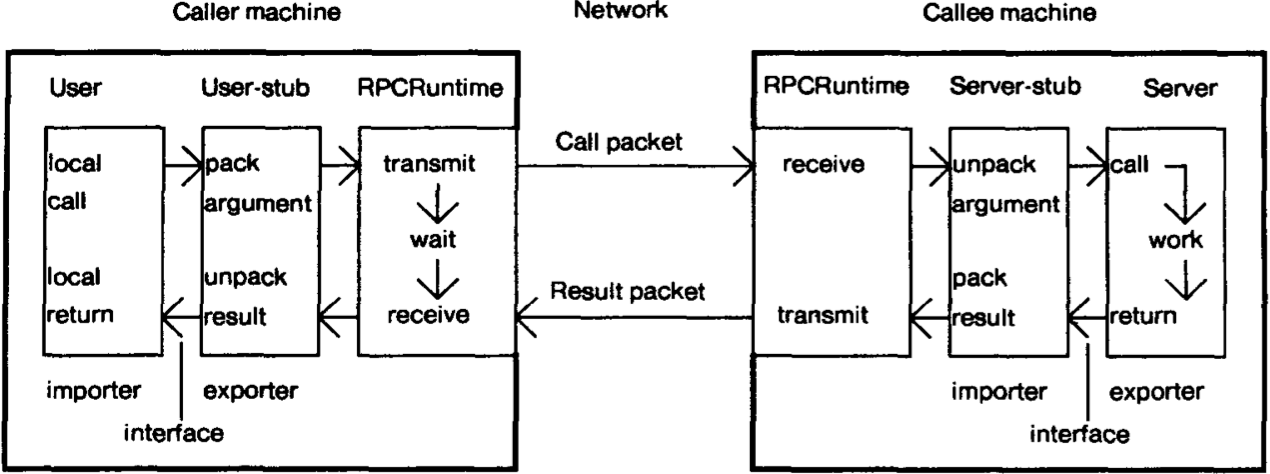
\includegraphics[width=\textwidth]{RPCDiagram_ImplementingRPC_ADBirrell_BJNelson.png} %uncomment to enable image
    \caption{The basic components of an RPC framework, from \cite{birrell1984implementing}}
    \label{fig:rpc-components}
\end{figure}

\subsection{The role of the RPCRuntime}
\label{RPCRuntimeBackgroundSection} 
The RPCRuntime is responsible for carrying out the actual communication of the RPC call information between the caller and the callee. It exists both in the caller and callee endpoints. When the caller makes a RPC call, the information is sent from the RPCRuntime sitting in the caller side, and is received by the RPCRuntime in the callee side. When the callee returns, the return data is sent from the callee's RPCRuntime to the caller's RPCRuntime.

In order to keep the context of a remote call, the RPCRuntime also sends some extra meta data along with the arguments. This meta data includes: 

\begin{enumerate}
	\item A call identifier. This is used for two reasons:
	\begin{enumerate}
		\item To check if the call has already been made (i.e. to ensure no duplicate calls)
		\item To match the return value of the callee with the correct caller.
	\end{enumerate}
	\item The name of the procedure the caller is calling.
	\item The arguments (parameters) we wish to pass to the remote procedure.
\end{enumerate}

The RPCRuntime on the caller side maintains a store of call identifiers that are currently in progress. When the remote functions return, they send the same call identifier along with the return value. That call identifier is then removed from the caller's store to indicate that the remote call has completed.


\section{Open Network Computing Remote Procedure Call}
\label{ONCRPCBackgroundSection} 
Open Network Computing (ONC) is a suite of software originally developed by Sun Microsystems. It provides a Remote Procedure Call (RPC) system along with an External Data Representation (XDR) format used alongside it. The ONC RPC system implements some tools and libraries that make it easy for developers to specify and use remote functions. These are:

\begin{enumerate}
	\item \textbf{RPCGen Compiler:} As mentioned earlier, the role of the user and server stubs is to pack and unpack arguments and results of function calls. To pack the arguments, the stub looks at the argument types and matches them with the number of arguments and their types of the server (callee) function definition. Thus, the stubs need to be written with knowledge of the interface of the actual procedures that will be called. We can define these interfaces in an abstract way, so that we could generate these stubs automatically even if the languages used in the different endpoints are different. In ONC RPC and many other systems, this abstract representation is in the form of an Interface Definition Language (IDL) file. When we pass the IDL file into the RPCGen compiler, it automatically generates the stubs we need to perform remote procedure calls.
	\item \textbf{XDR Routines:} These convert the types of the parameters and return values to and from the external data representation. XDR routines exist for many C types, and the system allows you to write your own XDR routines for complex types.
	\item \textbf{RPC API library:} This is an implementation that fulfils the role of the RPCRuntime described in \ref{RPCRuntimeBackgroundSection}. It provides a set of API functions that set up the lower level communication details, binding, and so on.
\end{enumerate}

Remote procedures in ONC RPC are identified by a program number, a version number, and a procedure number. There also exists a port mapper that map the program number to a port, so that several programs can run on the same remote machine. 

\subsection{Interface Definition Language files}
In ONC RPC, the XDR is used to define RPC definitions. For example, the RPC definition in listing \ref{samplerpc} defines an interface for a simple function that takes in a character string  and returns a structure containing two fields. As discussed in \ref{ONCRPCBackgroundSection}, we can see the program number is \verb+80000+ and the procedure number of the \verb+generate_keypair+ function is \verb+1+.

\lstset{language=c,caption={An example RPC definition for a key-pair generator function},label=samplerpc}
\begin{lstlisting}
/* File: keypairgen.x */
struct key_pair_t
{
  string  public_key<500>;
  string  private_key<500>;
};

program KEYPAIRGEN_PROGRAM
{
  version KEYPAIRGEN_VERSION
  {
    /* Produce a public/private key pair using a passphrase  */
    key_pair_t generate_keypair (string) = 1;
  } = 0;
} = 80000;
\end{lstlisting}

We can use the RPCGen compiler to then create client and server stubs. Passing the definition file \verb+keypairgen.x+ (shown in listing \ref{samplerpc}) into \verb+rpcgen+ will produce the following files:

\begin{itemize}
	\item \textbf{keypairgen.h} The header file, which would be included in both client and server code. Includes the actual C definition of the result\_t structure we defined in the XDR.
	\item \textbf{keypairgen\_clnt.c} The client stub, which packs the parameters and uses the RPC API library to execute the actual remote procedure call.
	\item \textbf{keypairgen\_svc.c} The server stub, which uses the RPC API to set up a listener for RPC calls. RPC calls are received, parameters are unpacked, and the actual function implementation (of \verb+generate_keypair+) is called.
	\item \textbf{keypairgen\_xdr.c} Defines methods for packing more complex structures, such as the \verb+key_pair_t+ structure we defined.
\end{itemize}

Now we need to write the actual implementation of the RPC procedure we wish to call remotely, namely \verb+generate_keypair+. This will include the generated header file and follow the specification we defined, as shown in listing \ref{samplerpcImp}. \\


\lstset{language=c,caption={An example server-side implementation of the procedure defined in \ref{samplerpc}},label=samplerpcImp}
\begin{lstlisting}
#include "keypairgen.h"

key_pair_t *
generate_keypair_0_svc(char **argp, struct svc_req *rqstp)
{
  static key_pair_t  result;
  // TODO: Actual implementation
  return(&result);
}
\end{lstlisting}

Finally, we call the remote procedure from the client, which includes the same header file and simply calls \verb+generate_keypair_0+, passing in the string parameter.



\section{WebIDL}
WebIDL is a new specification for an IDL that can be used by web browsers. It is used in several projects, including Google Chrome's Blink project http://www.chromium.org/blink/webidl 

This section is incomplete. Points I should mention:
\begin{itemize}
	\item WebIDL basics, using example
	\item How it can be used to generate C header files
	\item Existing implementations of C/C++ bindings (Including es OS). How bindings work?
	\item Parsers available
\end{itemize}

\textbf{Comment: } I'm actually not entirely sure I need this / how it can be used. NaCl already provides some functions to change types. I can use IDL to specify the functions I want to be available by RPC and what the parameters are. This will be used to generate stubs. The stubs use the NaCl functions available in the pp::Var class, such as AsDouble() to change types. Am I right? maybe I am getting confused as to what the IDL file is used for.

\section{Message Transfer}
This section is incomplete. Points I should mention:

\begin{itemize}
	\item NaCl allows representing data into any form. Examples are XDR or Protocol Buffers.
	\item Explain how the message format could increase performance
	\item Explain that the changing of message format is done in the client and server side stubs. This mean the message format will need to be supported in both JavaScript and NaCl
	\item Examine both XDR and protocol buffers
\end{itemize}

\textbf{Comment: } Technically, it is possible to do it all in JSON, right? Using protocol buffers for example is simply a way to improve performance.

 
%\chapter{Project \& Evaluation Plan} 

\label{Chapter3} 
\lhead{Chapter 3. \emph{Project \& Evaluation Plan}} 
% 	You should explain what needs to be done in order to complete the project and roughly what you expect the timetable to be. Don’t forget to include the project write-up, as this is a major part of the exercise. It’s important to identify key milestones and also fall-back positions, in case you run out of time.  You should also identify what extensions could be added if time permits.  The plan should be complete and should include those parts that you have already addressed (make it clear how far you have progressed at the time of writing).  This material will not appear in the final report.



\section{Project Key milestones}
\begin{description}
	\item[Implement NaClRPCGen] 
	~\\
	This is the main deliverable of the project. It will generate JavaScript and C++ header files using an input IDL file. These will be the stubs. This will consist of:
	\begin{itemize}
		\item Choosing a WebIDL parser. I will need to try out the existing parsers I have found and discussed in the WebIDL section of the background. Most likely, I will need to implement my own NaCl compatible WebIDL bindings, but I could definitely find inspiration from the C++ bindings. The JavaScript bindings are most likely going to be straight forward, but I will need to modify them so that they can call the library methods that will do the communications.
		\item Use the parser to create NaCl C++ bindings, and create JavaScript stub headers.
		\item Research and try out different message formats (some of which I have enumerated in the background). Find out what could be the best format to use. Perhaps some of them are useful for RPC over a network, where the main latency is the transferring of bytes, rather than format conversion.
		\item Most likely I will implement JSON-RPC just for simplicity. This could be a fallback.
	\end{itemize}
	\item[Implement the `RPCRuntime'] 
	~\\
	This will need to be done in both JavaScript and Native Client. This will be implemented on top of the message passing framework that already exists.
	\item[Give a working example]
	~\\
	Write an application that uses these tools, and show a typical development environment/cycle.
	\item[Write up] 
	~\\
	Complete the writeup to show how my RPC framework works, including the architecture and tools used. Give justification for each tool used, noting other alternatives I could have used.
\end{description}

\section{Implementation status \& plan}
Here is a preliminary timeline:

\begin{description}
	\item[February]
	~\\
	WebIDL parser should be ready, including deciding on JavaSript bindings and C++ bindings that I should base it on. A full system design should be made, which should explain the architecture of the RPC system. This should include the evaluation of different protocols and message formats.

	\item[March]
	~\\
	Parser should be developed and used to generate stubs. A first implementation of generating stubs (NaClRPCGen) should be done, and this should be a simple subset of the types supported by WebIDL. C++ header files and JavaScript functions should be automatically generated here. A first implementation of the RPCRuntime libraries should be started, and should allow basic remote procedure calls to the NaCl module.

	\item[April]
	~\\
	Iterative improvement of the parser, NaClRPCGen, and the RPCRuntime libraries. This should implement more and more types, and improve the RPC call framework. I should be able to use the RPC framework with different applications that already exist, such as bullet.

	\item[May and June]
	~\\
	Finish off implementation and complete the report, including evaluating the system (see Evaluation Plan). 

\end{description}

At the time of writing, none of these things have been implemented, as I spent time to research ideas and think of this plan. I plan to do a simple implementation this term that will include a parser and stub generator for very basic JavaScript and C++ types, e.g. just numbers. This exercise should help me understand how difficult it would be to do it for all types, and it would probably expose some areas I should think about in my architecture and implementation. I could come up with an incremental approach to implement the full product. This would ensure that even if the project is not completed by the deadline, I will at least have it working for \emph{some} types of programs.

\section{Evaluation Plan}
I think evaluation my project will include two types of evaluation, one quantitative and one qualitative.

The quantitative part includes measuring how much overhead the RPC framework adds to the simple message passing approach. I will need to measure this for different types of applications: e.g. applications which need to continuously call RPC functions might behave differently to applications which call them every once in a while.

The qualitative evaluation includes seeing how much development time is saved when using RPC. This could be measured by the number of lines the developer needs to write to achieve the same thing with message passing and with RPC.
%\input{Chapters/Chapter4} 
%\input{Chapters/Chapter5} 
%\input{Chapters/Chapter6} 
%\input{Chapters/Chapter7} 

%----------------------------------------------------------------------------------------
%	THESIS CONTENT - APPENDICES
%----------------------------------------------------------------------------------------

\addtocontents{toc}{\vspace{2em}} % Add a gap in the Contents, for aesthetics

%\appendix % Cue to tell LaTeX that the following 'chapters' are Appendices

% Include the appendices of the thesis as separate files from the Appendices folder
% Uncomment the lines as you write the Appendices

%% Appendix A

\chapter{Appendix Title Here} % Main appendix title

\label{AppendixA} % For referencing this appendix elsewhere, use \ref{AppendixA}

\lhead{Appendix A. \emph{Appendix Title Here}} % This is for the header on each page - perhaps a shortened title

Write your Appendix content here.
%\input{Appendices/AppendixB}
%\input{Appendices/AppendixC}

\addtocontents{toc}{\vspace{2em}} % Add a gap in the Contents, for aesthetics

\backmatter

%----------------------------------------------------------------------------------------
%	BIBLIOGRAPHY
%----------------------------------------------------------------------------------------

\label{Bibliography}

\lhead{\emph{Bibliography}} % Change the page header to say "Bibliography"

\bibliographystyle{unsrtnat} % Use the "unsrtnat" BibTeX style for formatting the Bibliography

\bibliography{Bibliography} % The references (bibliography) information are stored in the file named "Bibliography.bib"

\end{document}
